\documentclass[]{article}

\usepackage[left=2.00cm, right=2.00cm, top=2.00cm, bottom=2.00cm]{geometry}
\usepackage[spanish,es-noshorthands]{babel}
\usepackage[utf8]{inputenc} % para tildes y ñ
\usepackage{graphicx} % para las figuras
\usepackage{xcolor}
\usepackage{listings} % para el código fuente en c++

\lstdefinestyle{customc}{
  belowcaptionskip=1\baselineskip,
  breaklines=true,
  frame=single,
  xleftmargin=\parindent,
  language=C++,
  showstringspaces=false,
  basicstyle=\footnotesize\ttfamily,
  keywordstyle=\bfseries\color{green!40!black},
  commentstyle=\itshape\color{gray!40!gray},
  identifierstyle=\color{black},
  stringstyle=\color{orange},
}
\lstset{style=customc}


%opening
\title{Práctica 3. Divide y vencerás}
\author{Raúl Arcos Herrera \\ % mantenga las dos barras al final de la línea y este comentario
raul.arcosherrera@alum.uca.es\\ % mantenga las dos barras al final de la línea y este comentario
Teléfono: xxxxxxxx \\ % mantenga las dos barras al final de la linea y este comentario
NIF: 77175935X \\ % mantenga las dos barras al final de la línea y este comentario
}


\begin{document}

\maketitle

%\begin{abstract}
%\end{abstract}

% Ejemplo de ecuación a trozos
%
%$f(i,j)=\left\{ 
%  \begin{array}{lcr}
%      i + j & si & i < j \\ % caso 1
%      i + 7 & si & i = 1 \\ % caso 2
%      2 & si & i \geq j     % caso 3
%  \end{array}
%\right.$

\begin{enumerate}
\item Describa las estructuras de datos utilizados en cada caso para la representación del terreno de batalla. 

Escriba aquí su respuesta al ejercicio 1. 

% Elimine los símbolos de tanto por ciento para descomentar las siguientes instrucciones e incluir una imagen en su respuesta. La mejor ubicación de la imagen será determinada por el compilador de Latex. No tiene por qué situarse a continuación en el fichero en formato pdf resultante.
%\begin{figure}
%\centering
%\includegraphics[width=0.7\linewidth]{./defenseValueCellsHead} % no es necesario especificar la extensión del archivo que contiene la imagen
%\caption{Estrategia devoradora para la mina}
%\label{fig:defenseValueCellsHead}
%\end{figure}

En el caso del centro de extracción de minerales se han tenido en cuenta dos
factores valorar la mejor celda.
\begin{itemize}
    \item \textbf{Distancia respecto al centro} Se valorarán positivamente las celdas que se encuentren próximas al centro, 
    puesto que es el punto más alejado de la aparición de los UCOS.
    \item \textbf{Distancia respecto a obstáculos} Se valorará negativamente la cercanía
    a un obstáculo debido a que los obstáculos no protegen a las defensas de los proyectiles, por lo que es un entorpecimiento a la hora de hacer 
    formaciones en el mapa.
\end{itemize}

El valor final resulta de la ecuación: \textit{1000 - Distancia al centro / Factor de distancia a obstáculo}, siendo factor de distancia a obstáculo un número del 0 al 1, donde 0 es la completa ausencia de un obstáculo mientras que 1 es distancia cero con uno.
\\
Esto es así debido a que ese valor depende del tamaño del mapa, es decir, no es lo mismo tener un obstáculo a 20 unidades en un mapa de 40 que en un mapa de 100.


\item Implemente su propia versión del algoritmo de ordenación por fusión. Muestre a continuación el código fuente relevante. 

Codigo del algoritmo A Estrella utilizado:
\\
\begin{lstlisting}
//Para resolver esta practica utilizaremos el algoritmo A Estrella facilitado en las diapositivas del tema 4.

    AStarNode* current = originNode; //Cur
    std::vector<AStarNode*> o; //Opened
    std::vector<AStarNode*> c; //Closed
    bool found = false;

    current->G = 0;
    //estimatedDistance((cur,target) + additional cost)
    current->H = (estimatedDistance(current->position, targetNode->position)) + additionalCost[(int)(current->position.x/cellsWidth)][(int)(current->position.y/cellsHeight)];
    //std::cout << "ESTIMATED DISTANCE = " << current->H << std::endl;
    current->parent = NULL;
    current->F = current->G + current->H;

    //Comienzo del algoritmo A*
    o.push_back(current);
    std::make_heap(o.begin(), o.end(), condition);
    while(!found && !o.empty()){
        current = o.back();
        o.pop_back();
        c.push_back(current);
        if(current == targetNode)
            found = true;
        else{
            for(List<AStarNode*>::iterator it = current->adjacents.begin(); it != current->adjacents.end(); it++)
            {
                if(!perteneceNodo(c,(*it)))
                    if(!perteneceNodo(o,(*it))){
                        
                        (*it)->parent = current;
                        (*it)->G = current->G + estimatedDistance(current->position,(*it)->position);
                        (*it)->H = estimatedDistance((*it)->position, targetNode->position) + additionalCost[(int)(*it)->position.x/cellsWidth][(int)(*it)->position.y/cellsHeight];
                        (*it)->F = (*it)->G + (*it)->H;
                        o.push_back((*it));
                        std::make_heap(o.begin(), o.end(), condition);
                        std::sort_heap(o.begin(), o.end(), condition);
                    }
                    else
                        if((*it)->G > current->G + estimatedDistance(current->position, (*it)->position)){
                            
                            (*it)->parent = current;
                            (*it)->G = current->G + estimatedDistance(current->position, (*it)->position);
                            (*it)->F = (*it)->G + (*it)->H;
                            std::make_heap(o.begin(), o.end(), condition);
                            std::sort_heap(o.begin(), o.end(), condition);
                        }
            }
                
        }
    }
\end{lstlisting}



\item Implemente su propia versión del algoritmo de ordenación rápida. Muestre a continuación el código fuente relevante. 

\begin{lstlisting}
 //Compramos la primera defensa (Central)
    std::list<Defense*>::iterator currentDefense = defenses.begin();
    selectedIDs.push_back((*currentDefense)->id);
    ases-=(*currentDefense)->cost;
    currentDefense++;
    
    //Declaramos una matriz dinamica que usaremos como tabla de defensas-ases.
    float** table =  new float*[defenses.size()-1];
    //Creamos un vector para el coste (peso) de cada defensas
    int cost[defenses.size()-1];

    //Inicializamos tanto el vector de coste como la tabla TSR
    for(int i = 0; i < (defenses.size() - 1); i++)
    {
        table[i] = new float[ases];
        cost[i]=(*currentDefense)->cost;
        
        for(int j = 0; j < ases; j++)
            if(j < cost[i])
                //Si no es la primera defensa (Sin contar la central)
                if((*currentDefense)->id != 1) 
                    table[i][j] = table[i-1][j];
                else
                    table[i][j] = 0;  
            else 
                //Si no es la primera defensa (Sin contar la central)   
                if((*currentDefense)->id != 1)
                    table[i][j]=std::max(table[i-1][j], (table[i-1][j-cost[i]]+value((*currentDefense))));
                else
                    table[i][j] = value((*currentDefense));
        currentDefense++;
    }
\end{lstlisting}

\item Realice pruebas de caja negra para asegurar el correcto funcionamiento de los algoritmos de ordenación implementados en los ejercicios anteriores. Detalle a continuación el código relevante.

Para las pruebas de caja negra se ha utilizado el algoritmo voraz de la P1, básicamente rellenamos la estructura \textit{Cell} con los valores de cada celda por defecto y llamamos al procedimienton de ordenación correspondiente, después de eso utilizamos la función voraz de la P1 para colocar la mejor celda en el mapa y se mide el tiempo del proceso completo.
\\\\
Se utiliza a continuación como ejemplo la prueba de caja negra de la ordenación rápida.
\begin{lstlisting}
//TERCER METODO: ORDENACION RAPIDA.
    cronometro c3;
    long int r3 = 0;
    c3.activar();
    do{
        CellRapida(cell, 0, N-1);

       while(currentDefense != defenses.end()) {
            pos = voraz(freeCells,cell,nCellsWidth, nCellsHeight, mapWidth, mapHeight, obstacles, defenses, (*currentDefense)->radio,(*currentDefense)->id,N);
            (*currentDefense)->position.x = pos.x;
            (*currentDefense)->position.y = pos.y;
            (*currentDefense)->position.z = 0; 
            ++currentDefense;
        }	 
        ++r3;
    }while(c3.tiempo() < e_abs / e_rel + e_abs);
    c3.parar();
\end{lstlisting}

\item Analice de forma teórica la complejidad de las diferentes versiones del algoritmo de colocación de defensas en función de la estructura de representación del terreno de batalla elegida. Comente a continuación los resultados. Suponga un terreno de batalla cuadrado en todos los casos. 

Una vez colocado el centro de extracción, el valor otorgado al resto de defensas 
irá enfocado a rodear el centro de extracción.
\\
En mi caso, como se comenta brevemente en el punto anterior, otorgo el valor a las celdas con la función \textit{cellValue}, que 
mediante una flag determina si estamos colocando el centro de extracción o una simple defensa, 
por lo que una vez tenemos el centro de extracción en la posición (en mi  opinión) óptima, lo rodeamos de 
defensas para alargar lo máximo posible el alcance de los UCOS a esta.
\\
La ecuación para determinar el valor es la siguiente: \textit{value = 1000 - (distancia al centro de extracción)}.
\\
He elegido este método debido a que al rodear al centro, hay menos huecos que no entren en el radio de ataque de las defensas por los que puedan pasar los UCOS.


\item Incluya a continuación una gráfica con los resultados obtenidos. Utilice un esquema indirecto de medida (considere un error absoluto de valor 0.01 y un error relativo de valor 0.001). Considere en su análisis los planetas con códigos 1500, 2500, 3500,..., 10500. Incluya en el análisis los planetas que considere oportunos para mostrar información relevante.


\begin{figure}[!h]
        	\begin{centering}
        		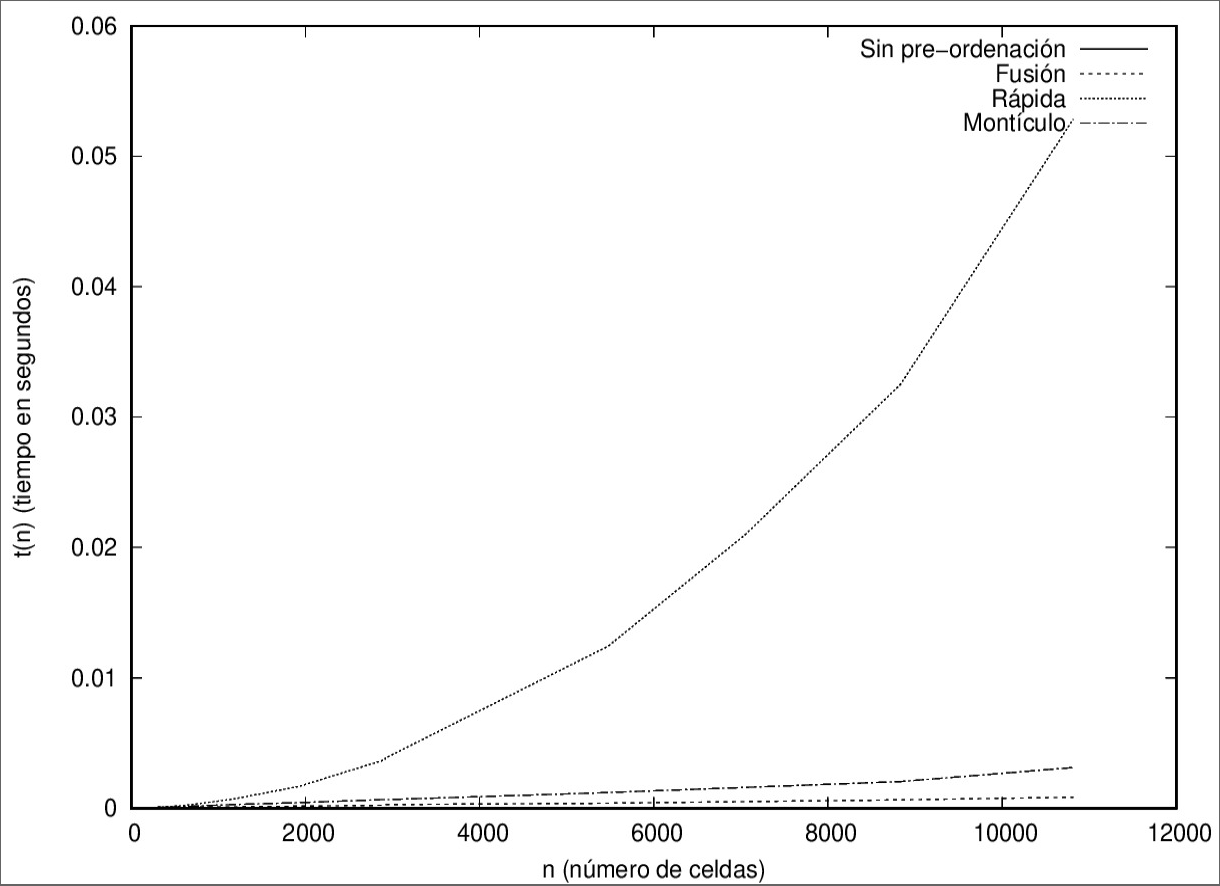
\includegraphics[width=0.8\textwidth]{grafica.png}
        		\label{fig:misComandos}
        	\end{centering}
\end{figure}

\end{enumerate}

Todo el material incluido en esta memoria y en los ficheros asociados es de mi autoría o ha sido facilitado por los profesores de la asignatura. Haciendo entrega de este documento confirmo que he leído la normativa de la asignatura, incluido el punto que respecta al uso de material no original.

\end{document}
